%!TeX root=../sensetop.tex
\chapter[Chapter \thechapter]{}
\lettrine[lines=4,lraise=0.3]{M}{rs} Palmer was so well at the end of a fortnight, that her mother felt it no longer necessary to give up the whole of her time to her; and, contenting herself with visiting her once or twice a day, returned from that period to her own home, and her own habits, in which she found the Miss Dashwoods very ready to resume their former share.

About the third or fourth morning after their being thus resettled in Berkeley Street, Mrs Jennings, on returning from her ordinary visit to Mrs Palmer, entered the drawing-room, where Elinor was sitting by herself, with an air of such hurrying importance as prepared her to hear something wonderful; and giving her time only to form that idea, began directly to justify it, by saying,

»Lord! my dear Miss Dashwood! have you heard the news?«

»No, ma’am. What is it?«

»Something so strange! But you shall hear it all. When I got to Mr Palmer’s, I found Charlotte quite in a fuss about the child. She was sure it was very ill—it cried, and fretted, and was all over pimples. So I looked at it directly, and, »Lord! my dear,« says I, »it is nothing in the world, but the red gum;« and nurse said just the same. But Charlotte, she would not be satisfied, so Mr Donavan was sent for; and luckily he happened to just come in from Harley Street, so he stepped over directly, and as soon as ever he saw the child, he said just as we did, that it was nothing in the world but the red gum, and then Charlotte was easy. And so, just as he was going away again, it came into my head, I am sure I do not know how I happened to think of it, but it came into my head to ask him if there was any news. So upon that, he smirked, and simpered, and looked grave, and seemed to know something or other, and at last he said in a whisper, »For fear any unpleasant report should reach the young ladies under your care as to their sister’s indisposition, I think it advisable to say, that I believe there is no great reason for alarm; I hope Mrs Dashwood will do very well.««

\begin{figure}[tbph]
\centering

\includegraphics[width=\linewidth]{37whisper}
\caption{In a whisper}
\end{figure}

»What! is Fanny ill?«

»That is exactly what I said, my dear. »Lord!« says I, »is Mrs Dashwood ill?« So then it all came out; and the long and the short of the matter, by all I can learn, seems to be this. Mr Edward Ferrars, the very young man I used to joke with you about (but however, as it turns out, I am monstrous glad there was never any thing in it), Mr Edward Ferrars, it seems, has been engaged above this twelvemonth to my cousin Lucy!—There’s for you, my dear! And not a creature knowing a syllable of the matter, except Nancy! Could you have believed such a thing possible? There is no great wonder in their liking one another; but that matters should be brought so forward between them, and nobody suspect it! \textit{That} is strange! I never happened to see them together, or I am sure I should have found it out directly. Well, and so this was kept a great secret, for fear of Mrs Ferrars, and neither she nor your brother or sister suspected a word of the matter: till this very morning, poor Nancy, who, you know, is a well-meaning creature, but no conjurer, popt it all out. »Lord!« thinks she to herself, »they are all so fond of Lucy, to be sure they will make no difficulty about it;« and so, away she went to your sister, who was sitting all alone at her carpet-work, little suspecting what was to come—for she had just been saying to your brother, only five minutes before, that she thought to make a match between Edward and some Lord’s daughter or other, I forget who. So you may think what a blow it was to all her vanity and pride. She fell into violent hysterics immediately, with such screams as reached your brother’s ears, as he was sitting in his own dressing-room down stairs, thinking about writing a letter to his steward in the country. So up he flew directly, and a terrible scene took place, for Lucy was come to them by that time, little dreaming what was going on. Poor soul! I pity \textit{her}. And I must say, I think she was used very hardly; for your sister scolded like any fury, and soon drove her into a fainting fit. Nancy, she fell upon her knees, and cried bitterly; and your brother, he walked about the room, and said he did not know what to do. Mrs Dashwood declared they should not stay a minute longer in the house, and your brother was forced to go down upon \textit{his} knees too, to persuade her to let them stay till they had packed up their clothes. \textit{Then} she fell into hysterics again, and he was so frightened that he would send for Mr Donavan, and Mr Donavan found the house in all this uproar. The carriage was at the door ready to take my poor cousins away, and they were just stepping in as he came off; poor Lucy in such a condition, he says, she could hardly walk; and Nancy, she was almost as bad. I declare, I have no patience with your sister; and I hope, with all my heart, it will be a match in spite of her. Lord! what a taking poor Mr Edward will be in when he hears of it! To have his love used so scornfully! for they say he is monstrous fond of her, as well he may. I should not wonder, if he was to be in the greatest passion!—and Mr Donavan thinks just the same. He and I had a great deal of talk about it; and the best of all is, that he is gone back again to Harley Street, that he may be within call when Mrs Ferrars is told of it, for she was sent for as soon as ever my cousins left the house, for your sister was sure \textit{she} would be in hysterics too; and so she may, for what I care. I have no pity for either of them. I have no notion of people’s making such a to-do about money and greatness. There is no reason on earth why Mr Edward and Lucy should not marry; for I am sure Mrs Ferrars may afford to do very well by her son, and though Lucy has next to nothing herself, she knows better than any body how to make the most of every thing; I dare say, if Mrs Ferrars would only allow him five hundred a-year, she would make as good an appearance with it as any body else would with eight. Lord! how snug they might live in such another cottage as yours—or a little bigger—with two maids, and two men; and I believe I could help them to a housemaid, for my Betty has a sister out of place, that would fit them exactly.«

Here Mrs Jennings ceased, and as Elinor had had time enough to collect her thoughts, she was able to give such an answer, and make such observations, as the subject might naturally be supposed to produce. Happy to find that she was not suspected of any extraordinary interest in it; that Mrs Jennings (as she had of late often hoped might be the case) had ceased to imagine her at all attached to Edward; and happy above all the rest, in the absence of Marianne, she felt very well able to speak of the affair without embarrassment, and to give her judgment, as she believed, with impartiality on the conduct of every one concerned in it.

She could hardly determine what her own expectation of its event really was; though she earnestly tried to drive away the notion of its being possible to end otherwise at last, than in the marriage of Edward and Lucy. What Mrs Ferrars would say and do, though there could not be a doubt of its nature, she was anxious to hear; and still more anxious to know how Edward would conduct himself. For \textit{him} she felt much compassion;—for Lucy very little—and it cost her some pains to procure that little;—for the rest of the party none at all.

As Mrs Jennings could talk on no other subject, Elinor soon saw the necessity of preparing Marianne for its discussion. No time was to be lost in undeceiving her, in making her acquainted with the real truth, and in endeavouring to bring her to hear it talked of by others, without betraying that she felt any uneasiness for her sister, or any resentment against Edward.

Elinor’s office was a painful one.—She was going to remove what she really believed to be her sister’s chief consolation,—to give such particulars of Edward as she feared would ruin him for ever in her good opinion,-and to make Marianne, by a resemblance in their situations, which to \textit{her} fancy would seem strong, feel all her own disappointment over again. But unwelcome as such a task must be, it was necessary to be done, and Elinor therefore hastened to perform it.

She was very far from wishing to dwell on her own feelings, or to represent herself as suffering much, any otherwise than as the self-command she had practised since her first knowledge of Edward’s engagement, might suggest a hint of what was practicable to Marianne. Her narration was clear and simple; and though it could not be given without emotion, it was not accompanied by violent agitation, nor impetuous grief. \textit{That} belonged rather to the hearer, for Marianne listened with horror, and cried excessively. Elinor was to be the comforter of others in her own distresses, no less than in theirs; and all the comfort that could be given by assurances of her own composure of mind, and a very earnest vindication of Edward from every charge but of imprudence, was readily offered.

But Marianne for some time would give credit to neither. Edward seemed a second Willoughby; and acknowledging as Elinor did, that she \textit{had} loved him most sincerely, could she feel less than herself! As for Lucy Steele, she considered her so totally unamiable, so absolutely incapable of attaching a sensible man, that she could not be persuaded at first to believe, and afterwards to pardon, any former affection of Edward for her. She would not even admit it to have been natural; and Elinor left her to be convinced that it was so, by that which only could convince her, a better knowledge of mankind.

Her first communication had reached no farther than to state the fact of the engagement, and the length of time it had existed.—Marianne’s feelings had then broken in, and put an end to all regularity of detail; and for some time all that could be done was to soothe her distress, lessen her alarms, and combat her resentment. The first question on her side, which led to farther particulars, was,—

»How long has this been known to you, Elinor? has he written to you?«

»I have known it these four months. When Lucy first came to Barton Park last November, she told me in confidence of her engagement.«

At these words, Marianne’s eyes expressed the astonishment which her lips could not utter. After a pause of wonder, she exclaimed—

»Four months!—Have you known of this four months?«

Elinor confirmed it.

»What! while attending me in all my misery, has this been on your heart? And I have reproached you for being happy!«

»It was not fit that you should then know how much I was the reverse!«

»Four months!« cried Marianne again. »So calm! so cheerful! How have you been supported?«

»By feeling that I was doing my duty.—My promise to Lucy, obliged me to be secret. I owed it to her, therefore, to avoid giving any hint of the truth; and I owed it to my family and friends, not to create in them a solicitude about me, which it could not be in my power to satisfy.«

Marianne seemed much struck.

»I have very often wished to undeceive yourself and my mother,« added Elinor; »and once or twice I have attempted it;—but without betraying my trust, I never could have convinced you.«

»Four months! and yet you loved him!«

»Yes. But I did not love only him; and while the comfort of others was dear to me, I was glad to spare them from knowing how much I felt. Now, I can think and speak of it with little emotion. I would not have you suffer on my account; for I assure you I no longer suffer materially myself. I have many things to support me. I am not conscious of having provoked the disappointment by any imprudence of my own, I have borne it as much as possible without spreading it farther. I acquit Edward of essential misconduct. I wish him very happy; and I am so sure of his always doing his duty, that though now he may harbour some regret, in the end he must become so. Lucy does not want sense, and that is the foundation on which every thing good may be built. And after all, Marianne, after all that is bewitching in the idea of a single and constant attachment, and all that can be said of one’s happiness depending entirely on any particular person, it is not meant—it is not fit—it is not possible that it should be so. Edward will marry Lucy; he will marry a woman superior in person and understanding to half her sex; and time and habit will teach him to forget that he ever thought another superior to \textit{her}.«

»If such is your way of thinking,« said Marianne, »if the loss of what is most valued is so easily to be made up by something else, your resolution, your self-command, are, perhaps, a little less to be wondered at.—They are brought more within my comprehension.«

»I understand you. You do not suppose that I have ever felt much. For four months, Marianne, I have had all this hanging on my mind, without being at liberty to speak of it to a single creature; knowing that it would make you and my mother most unhappy whenever it were explained to you, yet unable to prepare you for it in the least. It was told me,—it was in a manner forced on me by the very person herself, whose prior engagement ruined all my prospects; and told me, as I thought, with triumph. This person’s suspicions, therefore, I have had to oppose, by endeavouring to appear indifferent where I have been most deeply interested; and it has not been only once; I have had her hopes and exultation to listen to again and again. I have known myself to be divided from Edward for ever, without hearing one circumstance that could make me less desire the connection. Nothing has proved him unworthy; nor has anything declared him indifferent to me. I have had to contend against the unkindness of his sister, and the insolence of his mother; and have suffered the punishment of an attachment, without enjoying its advantages. And all this has been going on at a time, when, as you know too well, it has not been my only unhappiness. If you can think me capable of ever feeling, surely you may suppose that I have suffered \textit{now}. The composure of mind with which I have brought myself at present to consider the matter, the consolation that I have been willing to admit, have been the effect of constant and painful exertion; they did not spring up of themselves; they did not occur to relieve my spirits at first. No, Marianne. \textit{Then}, if I had not been bound to silence, perhaps nothing could have kept me entirely—not even what I owed to my dearest friends—from openly showing that I was \textit{very} unhappy.«

Marianne was quite subdued.

»Oh! Elinor,« she cried, »you have made me hate myself for ever.—How barbarous have I been to you!—you, who have been my only comfort, who have borne with me in all my misery, who have seemed to be only suffering for me!—Is this my gratitude?—Is this the only return I can make you?—Because your merit cries out upon myself, I have been trying to do it away.«

The tenderest caresses followed this confession. In such a frame of mind as she was now in, Elinor had no difficulty in obtaining from her whatever promise she required; and at her request, Marianne engaged never to speak of the affair to any one with the least appearance of bitterness; to meet Lucy without betraying the smallest increase of dislike to her; and even to see Edward himself, if chance should bring them together, without any diminution of her usual cordiality. These were great concessions; but where Marianne felt that she had injured, no reparation could be too much for her to make.

She performed her promise of being discreet, to admiration.—She attended to all that Mrs Jennings had to say upon the subject, with an unchanging complexion, dissented from her in nothing, and was heard three times to say, »Yes, ma’am.«—She listened to her praise of Lucy with only moving from one chair to another, and when Mrs Jennings talked of Edward’s affection, it cost her only a spasm in her throat.—Such advances towards heroism in her sister, made Elinor feel equal to any thing herself.

The next morning brought a farther trial of it, in a visit from their brother, who came with a most serious aspect to talk over the dreadful affair, and bring them news of his wife.

»You have heard, I suppose,« said he with great solemnity, as soon as he was seated, »of the very shocking discovery that took place under our roof yesterday.«

\begin{a4}
	\begin{figure}[tbph]
		\centering
		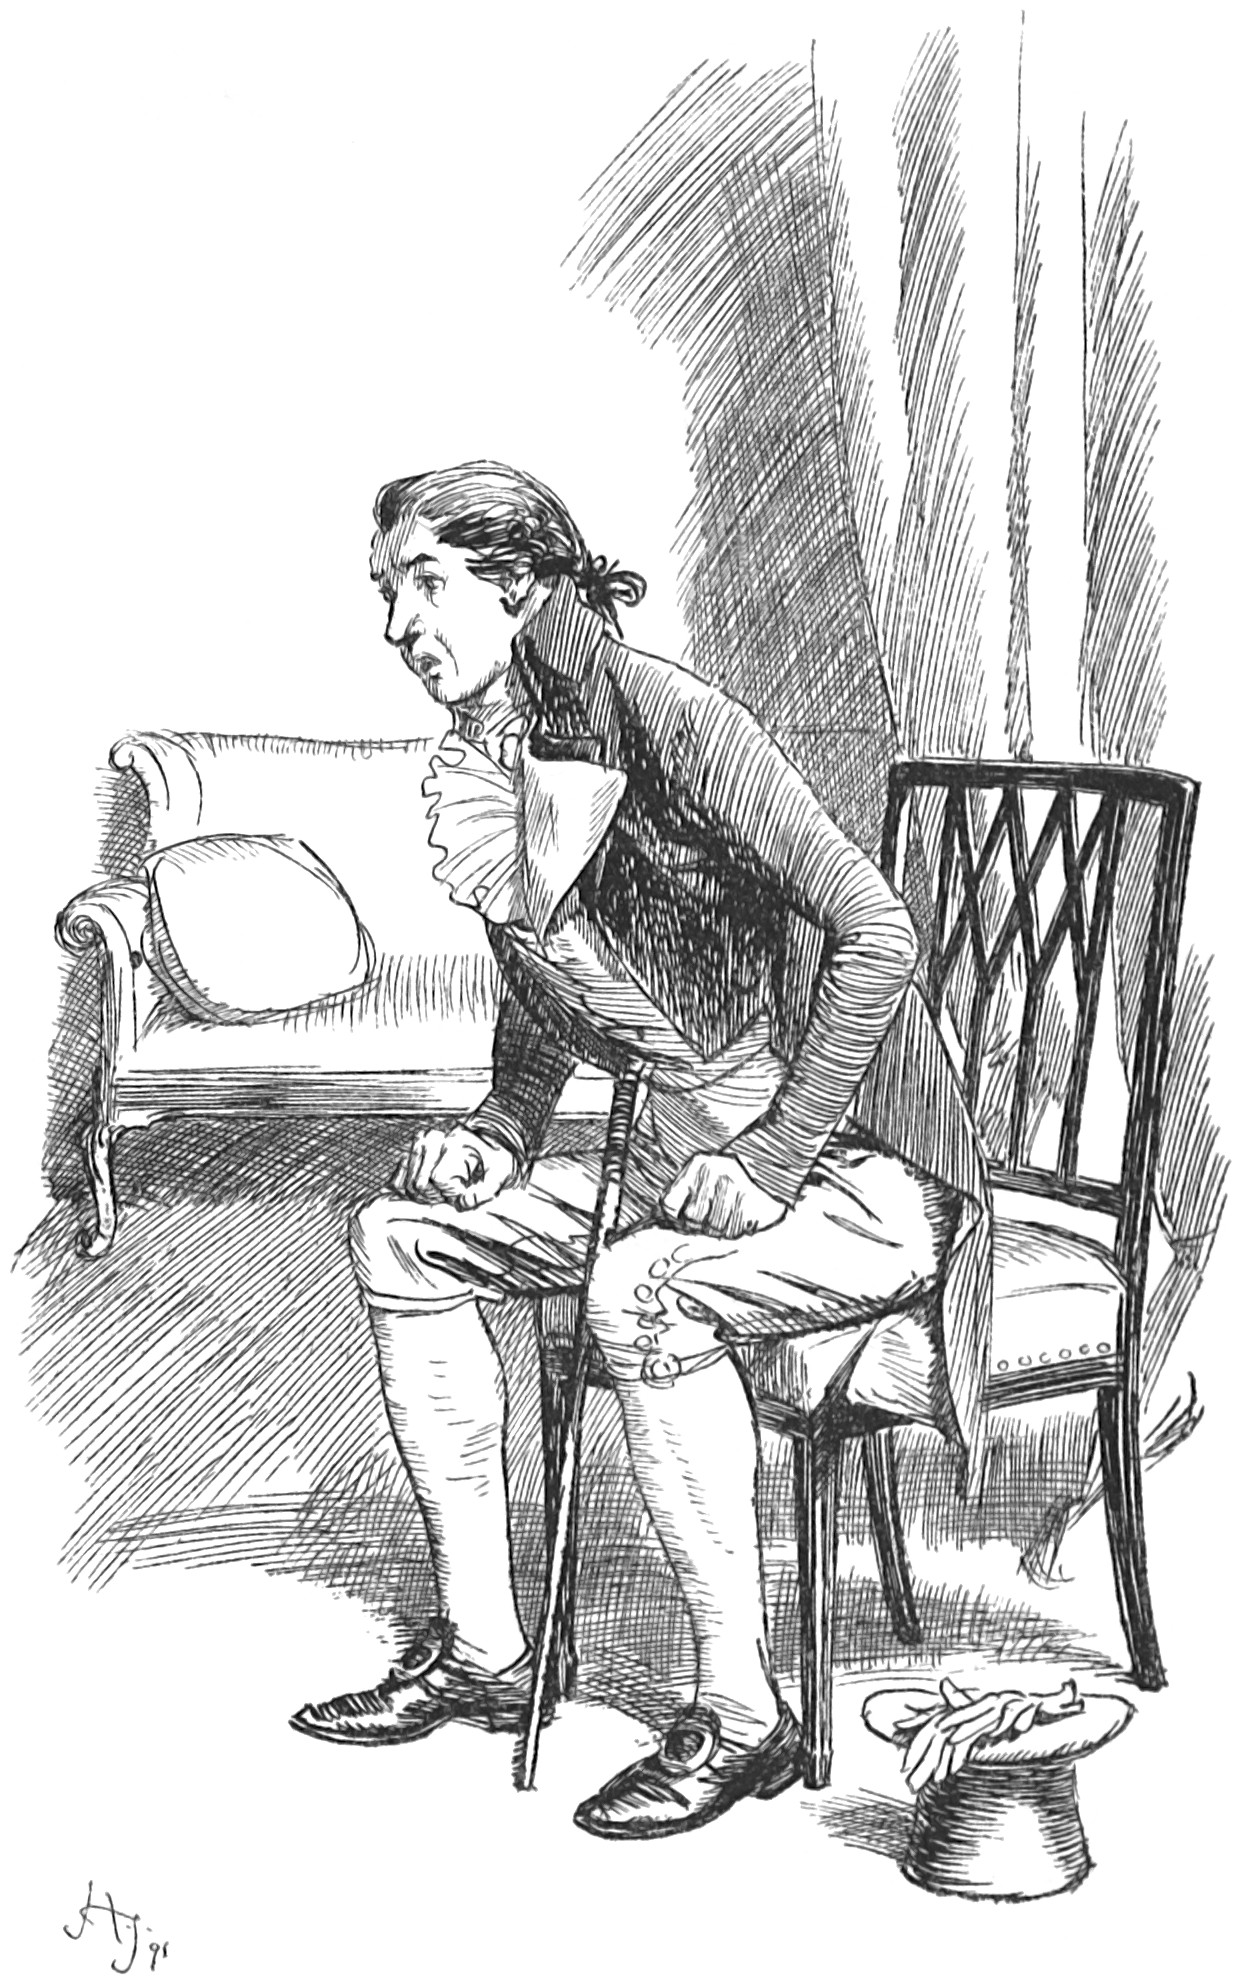
\includegraphics[width=.9\linewidth]{37haveheard}
		\caption{»You have heard, I suppose«}
	\end{figure}
\end{a4}

\begin{letter}
	\begin{figure}[tbph]
		\centering
		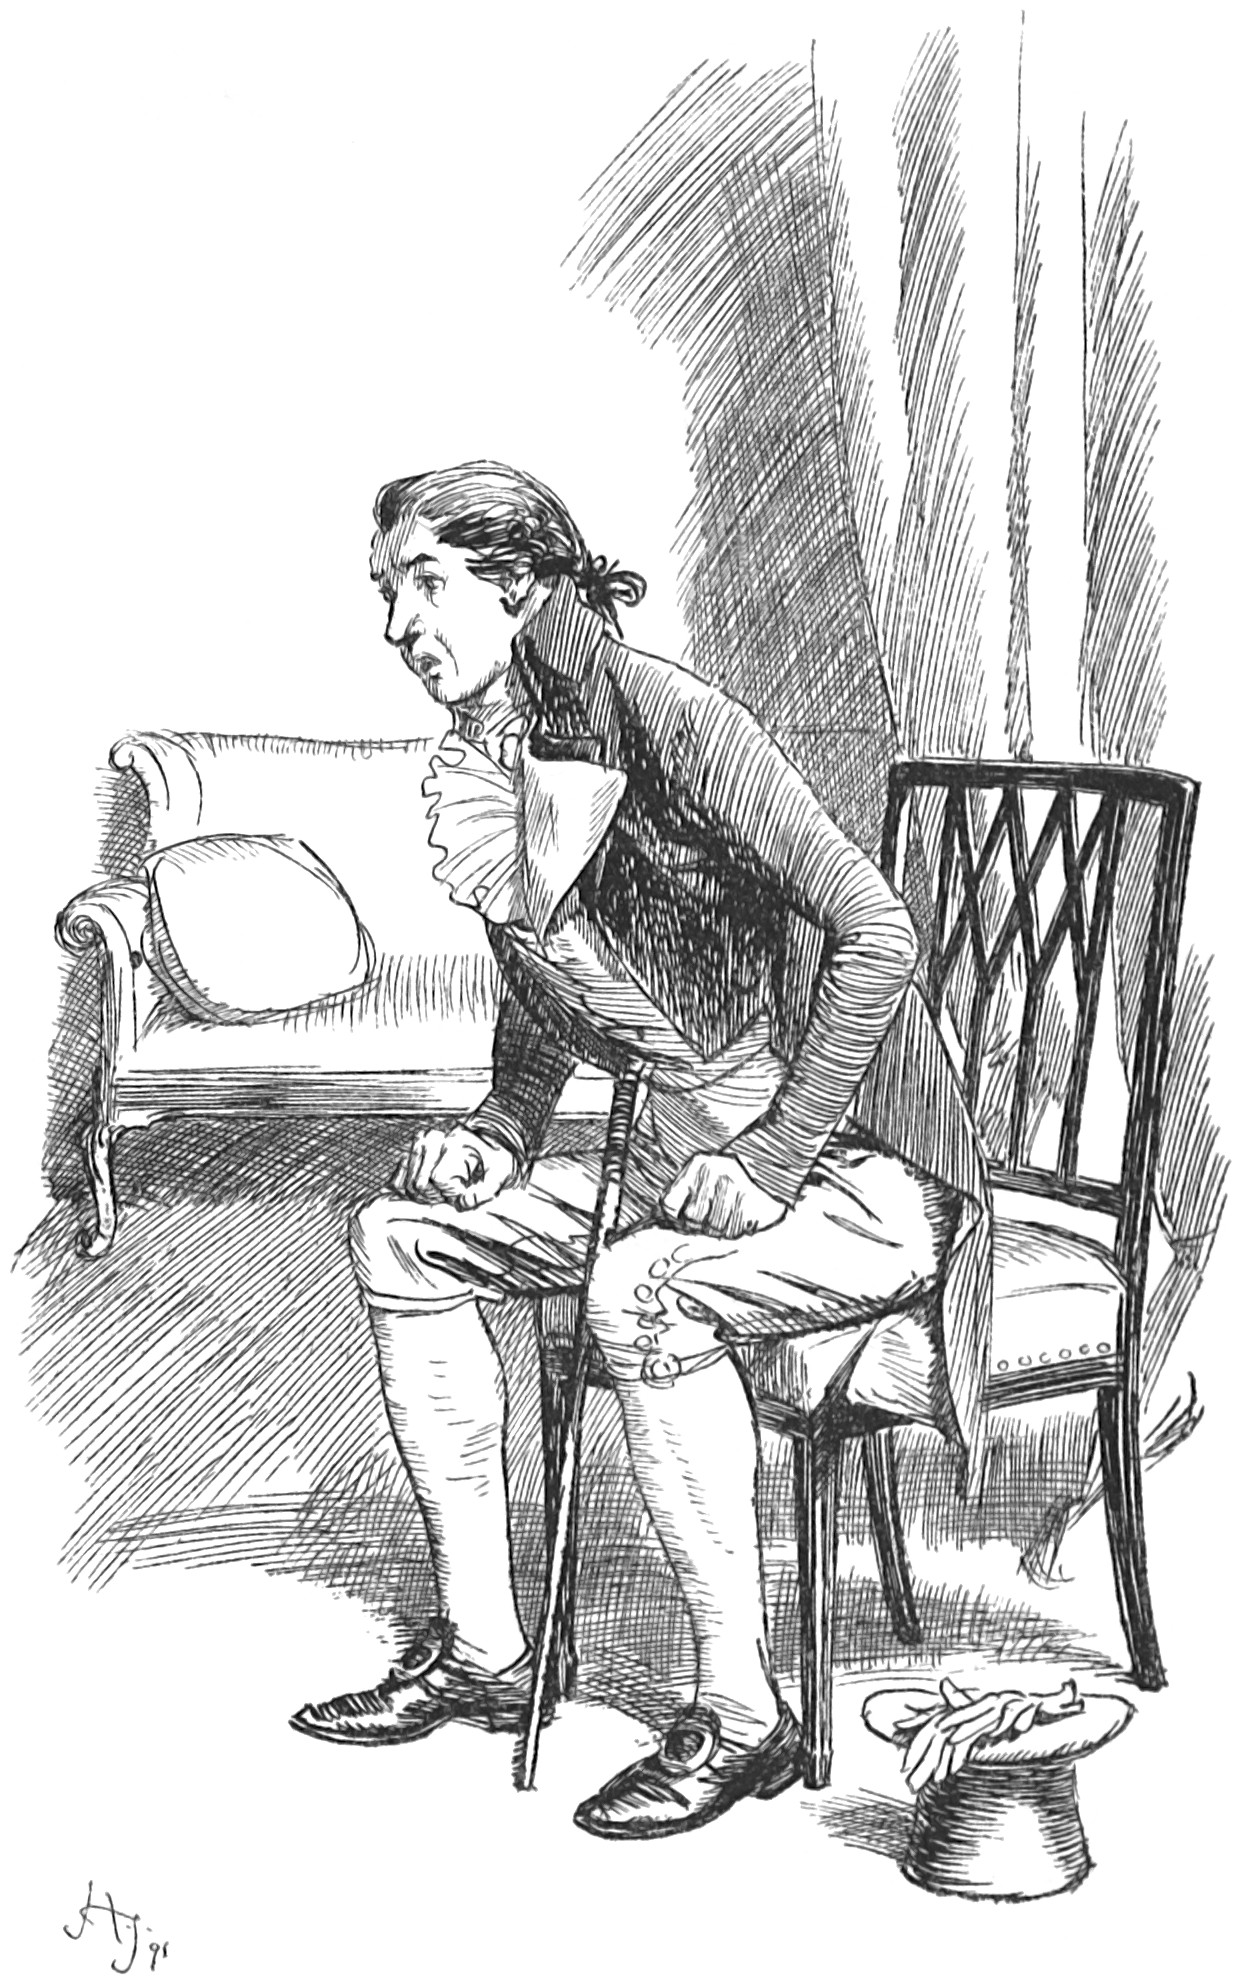
\includegraphics[width=\linewidth]{37haveheard}
		\caption{»You have heard, I suppose«}
	\end{figure}
\end{letter}

They all looked their assent; it seemed too awful a moment for speech.

»Your sister,« he continued, »has suffered dreadfully. Mrs Ferrars too—in short it has been a scene of such complicated distress—but I will hope that the storm may be weathered without our being any of us quite overcome. Poor Fanny! she was in hysterics all yesterday. But I would not alarm you too much. Donavan says there is nothing materially to be apprehended; her constitution is a good one, and her resolution equal to any thing. She has borne it all, with the fortitude of an angel! She says she never shall think well of anybody again; and one cannot wonder at it, after being so deceived!—meeting with such ingratitude, where so much kindness had been shown, so much confidence had been placed! It was quite out of the benevolence of her heart, that she had asked these young women to her house; merely because she thought they deserved some attention, were harmless, well-behaved girls, and would be pleasant companions; for otherwise we both wished very much to have invited you and Marianne to be with us, while your kind friend there, was attending her daughter. And now to be so rewarded! »I wish, with all my heart,« says poor Fanny in her affectionate way, »that we had asked your sisters instead of them.««

Here he stopped to be thanked; which being done, he went on.

»What poor Mrs Ferrars suffered, when first Fanny broke it to her, is not to be described. While she with the truest affection had been planning a most eligible connection for him, was it to be supposed that he could be all the time secretly engaged to another person!—such a suspicion could never have entered her head! If she suspected \textit{any} prepossession elsewhere, it could not be in \textit{that} quarter. »\textit{There}, to be sure,« said she, »I might have thought myself safe.« She was quite in an agony. We consulted together, however, as to what should be done, and at last she determined to send for Edward. He came. But I am sorry to relate what ensued. All that Mrs Ferrars could say to make him put an end to the engagement, assisted too as you may well suppose by my arguments, and Fanny’s entreaties, was of no avail. Duty, affection, every thing was disregarded. I never thought Edward so stubborn, so unfeeling before. His mother explained to him her liberal designs, in case of his marrying Miss Morton; told him she would settle on him the Norfolk estate, which, clear of land-tax, brings in a good thousand a-year; offered even, when matters grew desperate, to make it twelve hundred; and in opposition to this, if he still persisted in this low connection, represented to him the certain penury that must attend the match. His own two thousand pounds she protested should be his all; she would never see him again; and so far would she be from affording him the smallest assistance, that if he were to enter into any profession with a view of better support, she would do all in her power to prevent him advancing in it.«

Here Marianne, in an ecstasy of indignation, clapped her hands together, and cried, »Gracious God! can this be possible!«

»Well may you wonder, Marianne,« replied her brother, »at the obstinacy which could resist such arguments as these. Your exclamation is very natural.«

Marianne was going to retort, but she remembered her promises, and forbore.

»All this, however,« he continued, »was urged in vain. Edward said very little; but what he did say, was in the most determined manner. Nothing should prevail on him to give up his engagement. He would stand to it, cost him what it might.«

»Then,« cried Mrs Jennings with blunt sincerity, no longer able to be silent, »he has acted like an honest man! I beg your pardon, Mr Dashwood, but if he had done otherwise, I should have thought him a rascal. I have some little concern in the business, as well as yourself, for Lucy Steele is my cousin, and I believe there is not a better kind of girl in the world, nor one who more deserves a good husband.«

John Dashwood was greatly astonished; but his nature was calm, not open to provocation, and he never wished to offend anybody, especially anybody of good fortune. He therefore replied, without any resentment,

»I would by no means speak disrespectfully of any relation of yours, madam. Miss Lucy Steele is, I dare say, a very deserving young woman, but in the present case you know, the connection must be impossible. And to have entered into a secret engagement with a young man under her uncle’s care, the son of a woman especially of such very large fortune as Mrs Ferrars, is perhaps, altogether a little extraordinary. In short, I do not mean to reflect upon the behaviour of any person whom you have a regard for, Mrs Jennings. We all wish her extremely happy; and Mrs Ferrars’s conduct throughout the whole, has been such as every conscientious, good mother, in like circumstances, would adopt. It has been dignified and liberal. Edward has drawn his own lot, and I fear it will be a bad one.«

Marianne sighed out her similar apprehension; and Elinor’s heart wrung for the feelings of Edward, while braving his mother’s threats, for a woman who could not reward him.

»Well, sir,« said Mrs Jennings, »and how did it end?«

»I am sorry to say, ma’am, in a most unhappy rupture:—Edward is dismissed for ever from his mother’s notice. He left her house yesterday, but where he is gone, or whether he is still in town, I do not know; for \textit{we} of course can make no inquiry.«

»Poor young man!—and what is to become of him?«

»What, indeed, ma’am! It is a melancholy consideration. Born to the prospect of such affluence! I cannot conceive a situation more deplorable. The interest of two thousand pounds—how can a man live on it?—and when to that is added the recollection, that he might, but for his own folly, within three months have been in the receipt of two thousand, five hundred a-year (for Miss Morton has thirty thousand pounds,) I cannot picture to myself a more wretched condition. We must all feel for him; and the more so, because it is totally out of our power to assist him.«

»Poor young man!« cried Mrs Jennings, »I am sure he should be very welcome to bed and board at my house; and so I would tell him if I could see him. It is not fit that he should be living about at his own charge now, at lodgings and taverns.«

Elinor’s heart thanked her for such kindness towards Edward, though she could not forbear smiling at the form of it.

»If he would only have done as well by himself,« said John Dashwood, »as all his friends were disposed to do by him, he might now have been in his proper situation, and would have wanted for nothing. But as it is, it must be out of anybody’s power to assist him. And there is one thing more preparing against him, which must be worse than all—his mother has determined, with a very natural kind of spirit, to settle \textit{that} estate upon Robert immediately, which might have been Edward’s, on proper conditions. I left her this morning with her lawyer, talking over the business.«

\begin{figure}[tbph]
\centering

\includegraphics[width=\linewidth]{37talking}
\caption{Talking over the business}
\end{figure}

»Well!« said Mrs Jennings, »that is \textit{her} revenge. Everybody has a way of their own. But I don’t think mine would be, to make one son independent, because another had plagued me.«

Marianne got up and walked about the room.

»Can anything be more galling to the spirit of a man,« continued John, »than to see his younger brother in possession of an estate which might have been his own? Poor Edward! I feel for him sincerely.«

A few minutes more spent in the same kind of effusion, concluded his visit; and with repeated assurances to his sisters that he really believed there was no material danger in Fanny’s indisposition, and that they need not therefore be very uneasy about it, he went away; leaving the three ladies unanimous in their sentiments on the present occasion, as far at least as it regarded Mrs Ferrars’s conduct, the Dashwoods’, and Edward’s.

Marianne’s indignation burst forth as soon as he quitted the room; and as her vehemence made reserve impossible in Elinor, and unnecessary in Mrs Jennings, they all joined in a very spirited critique upon the party.